\section{Resultados}

Para analizar los datos, en primer lugar tomamos una muestra aleatoria de 10 pares de números enteros $(x,y)$ entre 0 y 10, para esto usamos un generador de números aleatorio. Con este set de datos y un $\Delta$ de $0.5$, llamado \textit{random\_ints.txt}, lo pasamos como parámetro a las tres funciones de spline (uniforme, chord-length y centrípeta). Las constantes ERROR y CANT\_SIMPSON fueron escogidas en 0.1 y 6 respectivamente.

Para poder observar la curva descripta por el spline, usamos como base los vectores impresos a intervalos $t = 0.1$, esto obviamente sabemos que no nos va a dar la curva del spline exacta, pero nos va a permitir aproximarla de manera suficientemente exacta sin que ello conlleve un gran costo de cálculo.

Por lo tanto, teniendo la curva del spline graficada, hicimos diferentes gráficos que mostraran la parametrización sobre $\Delta * i$ y la reparametrización, para cada tipo de parametrización.



\begin{center}
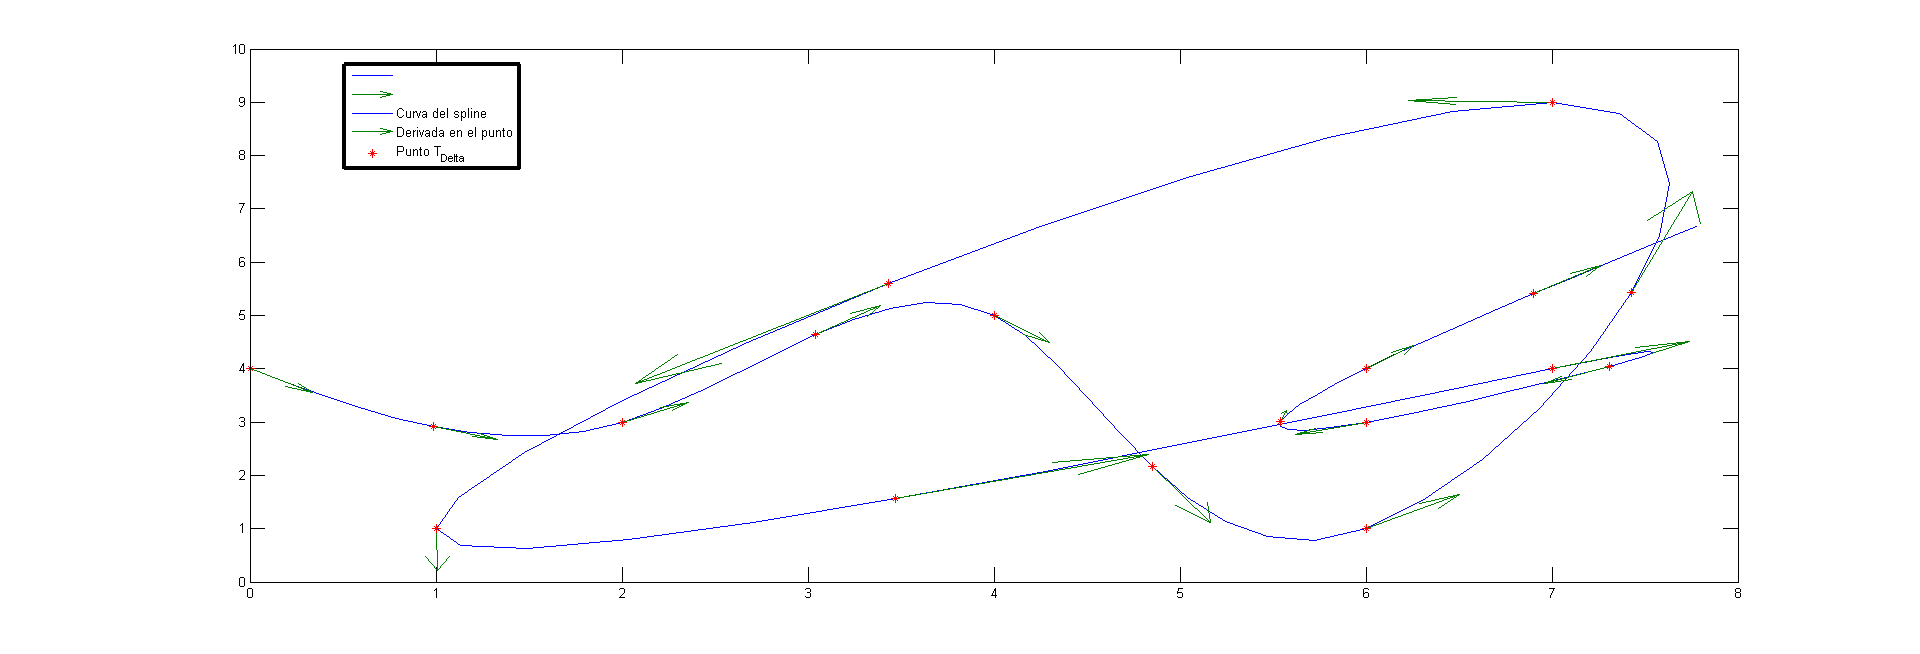
\includegraphics[scale=0.4]{../img/Uniforme-orig-rand.png} \\
\scriptsize{\textsf{\textbf{Gr\'afico 1.1, Spline y parametrización original dada una parametrización uniforme de los puntos sampleados, con puntos de entrada al azar}}}
\end{center}

\begin{center}
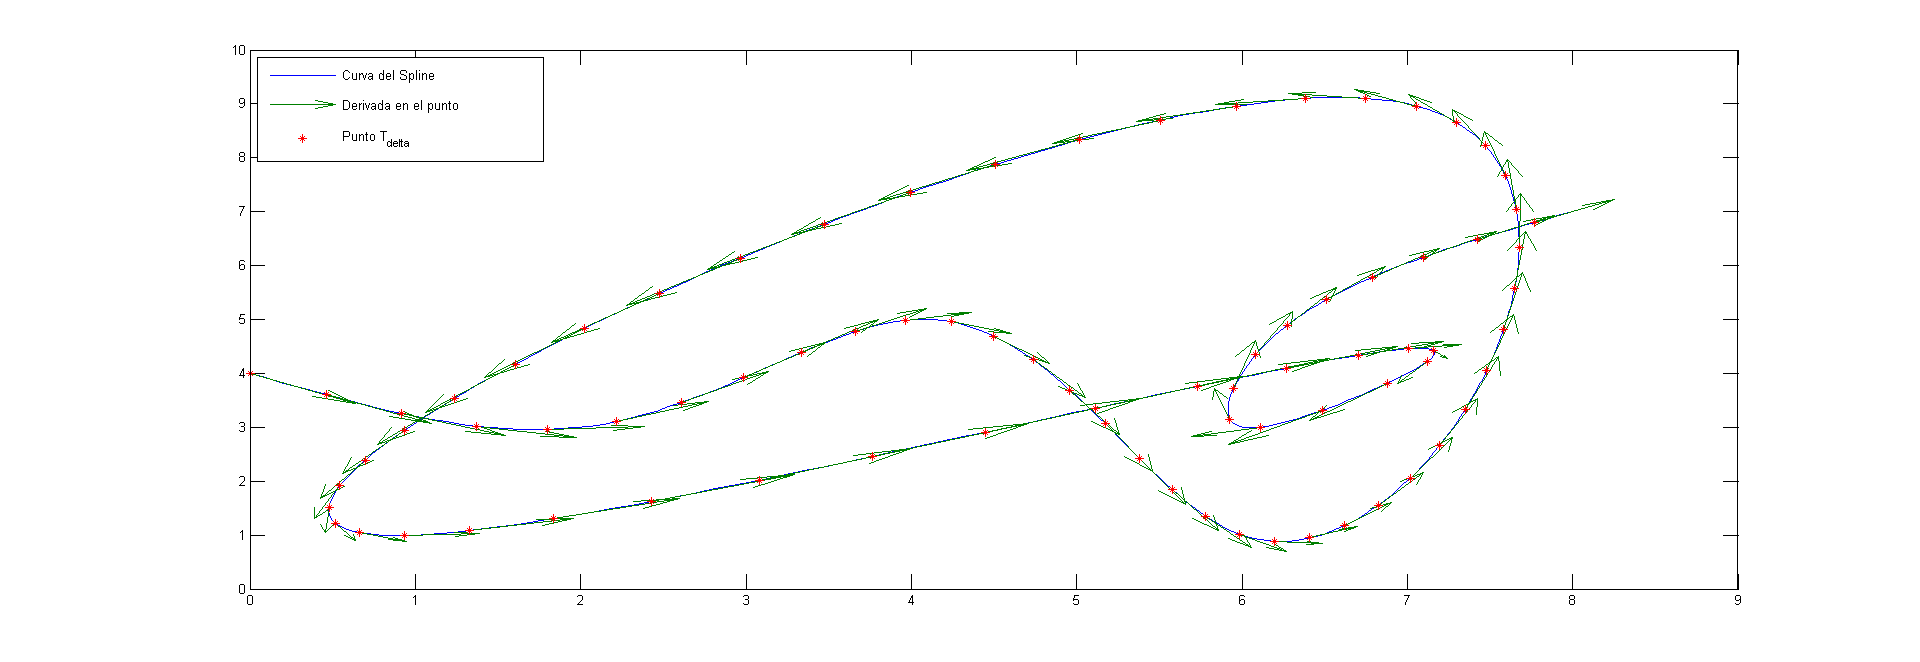
\includegraphics[scale=0.4]{../img/Chord-orig-rand.png} \\
\scriptsize{\textsf{\textbf{Gr\'afico 1.2, Spline y parametrización original dada una parametrización chord-length de los puntos sampleados, con puntos de entrada al azar}}}
\end{center}

\begin{center}
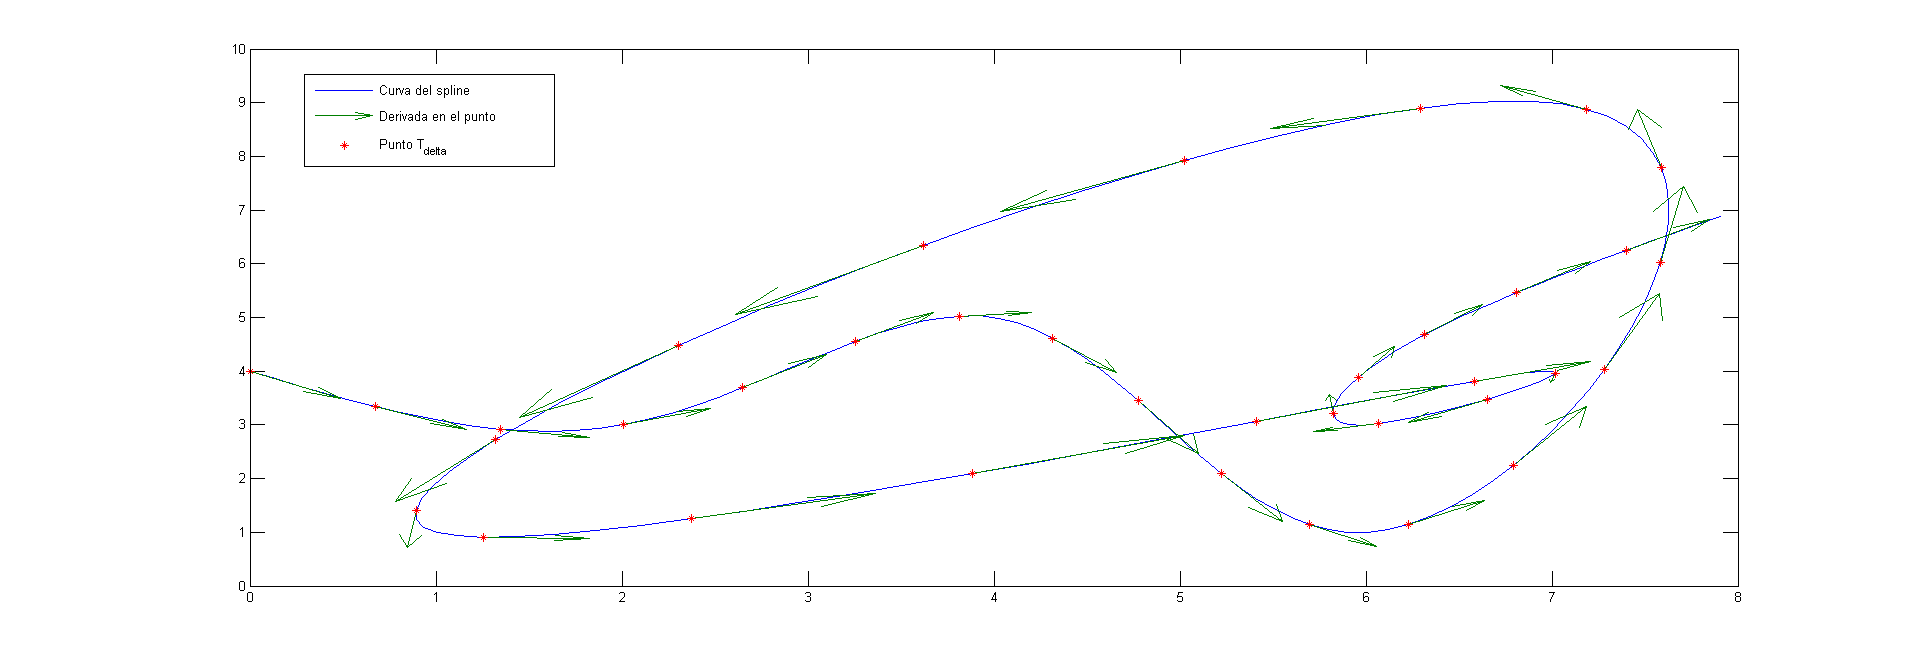
\includegraphics[scale=0.4]{../img/Centripeta-orig-rand.png} \\
\scriptsize{\textsf{\textbf{Gr\'afico 1.3, Spline y parametrización original dada una parametrización centrípeta de los puntos sampleados, con puntos de entrada al azar}}}
\end{center}


Luego, se usó la reparametrización, con el mismo set de puntos y el mismo delta, para obtener nuevos datos.


\begin{center}
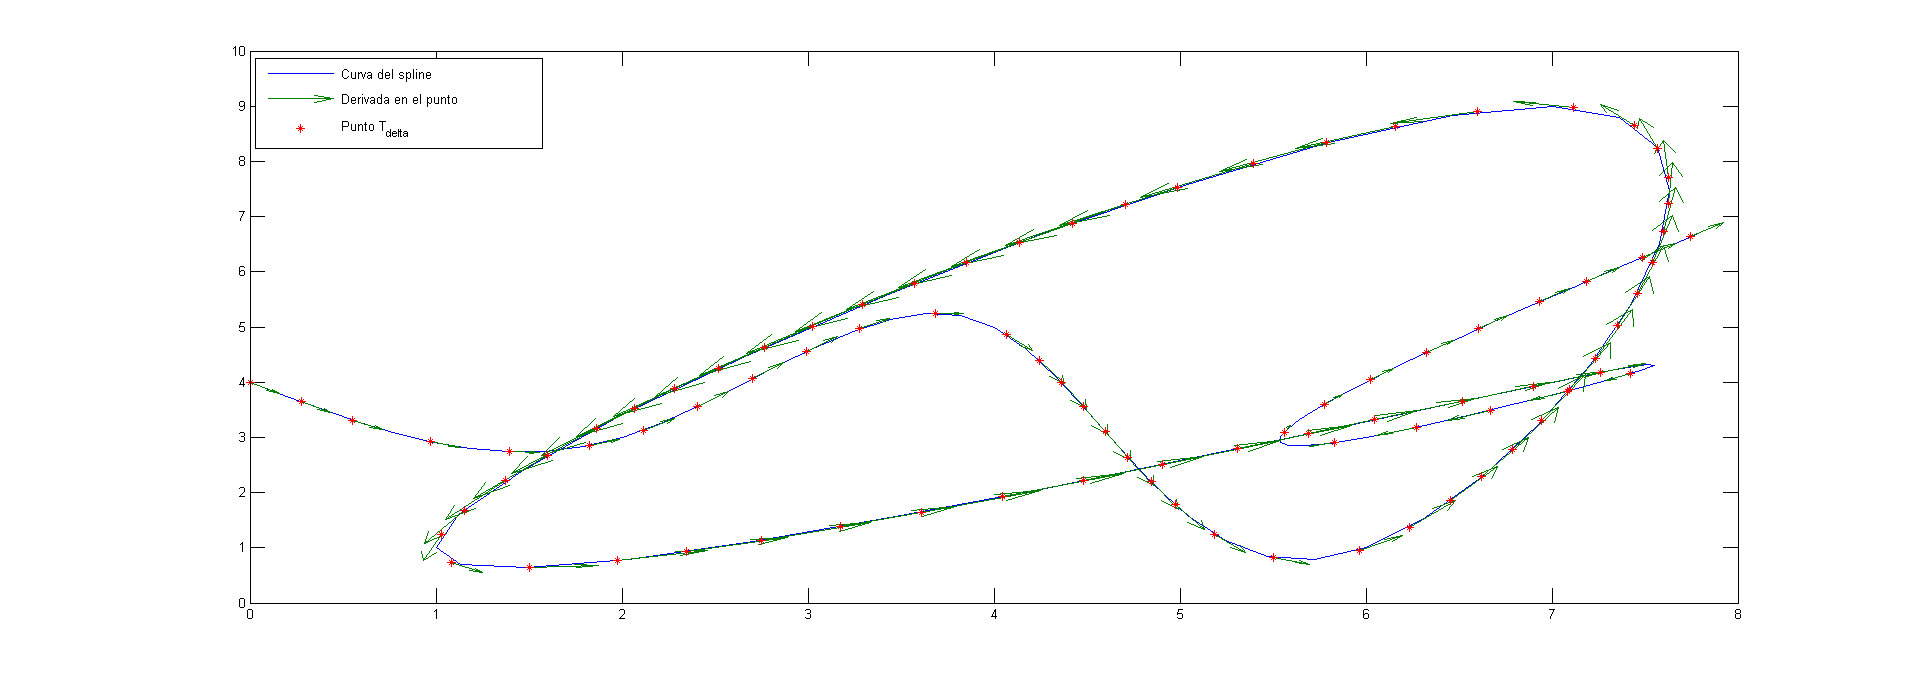
\includegraphics[scale=0.4]{../img/Uniforme-repa-rand.png} \\
\scriptsize{\textsf{\textbf{Gr\'afico 2.1, Spline y reparametrización dada una parametrización uniforme de los puntos sampleados, con puntos de entrada al azar}}}
\end{center}

\begin{center}
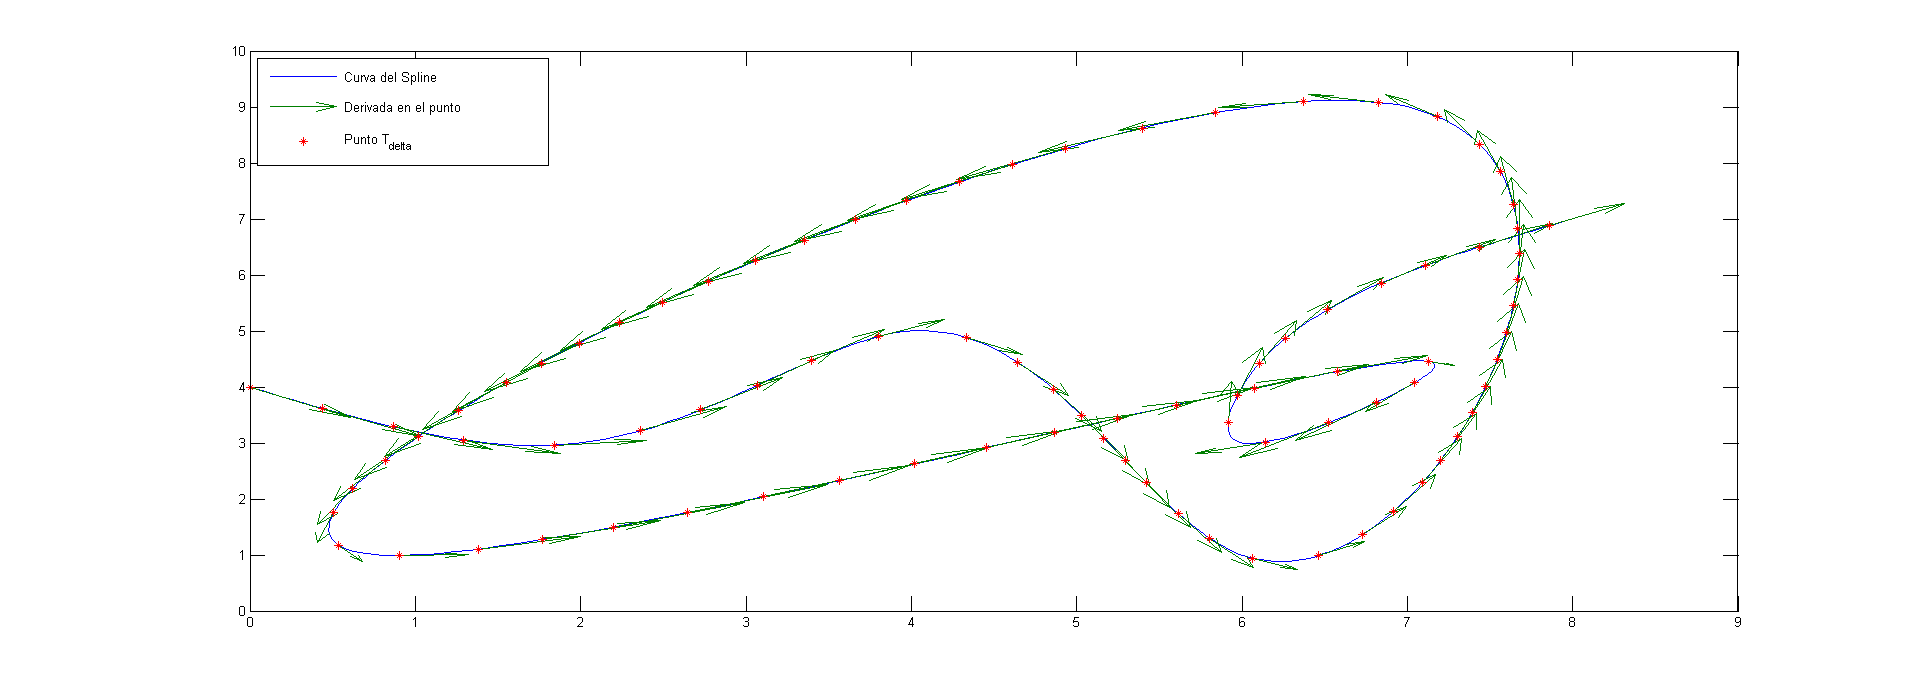
\includegraphics[scale=0.4]{../img/Chord-repa-rand.png} \\
\scriptsize{\textsf{\textbf{Gr\'afico 2.2, Spline y reparametrización dada una parametrización chord-length de los puntos sampleados, con puntos de entrada al azar}}}
\end{center}

\begin{center}
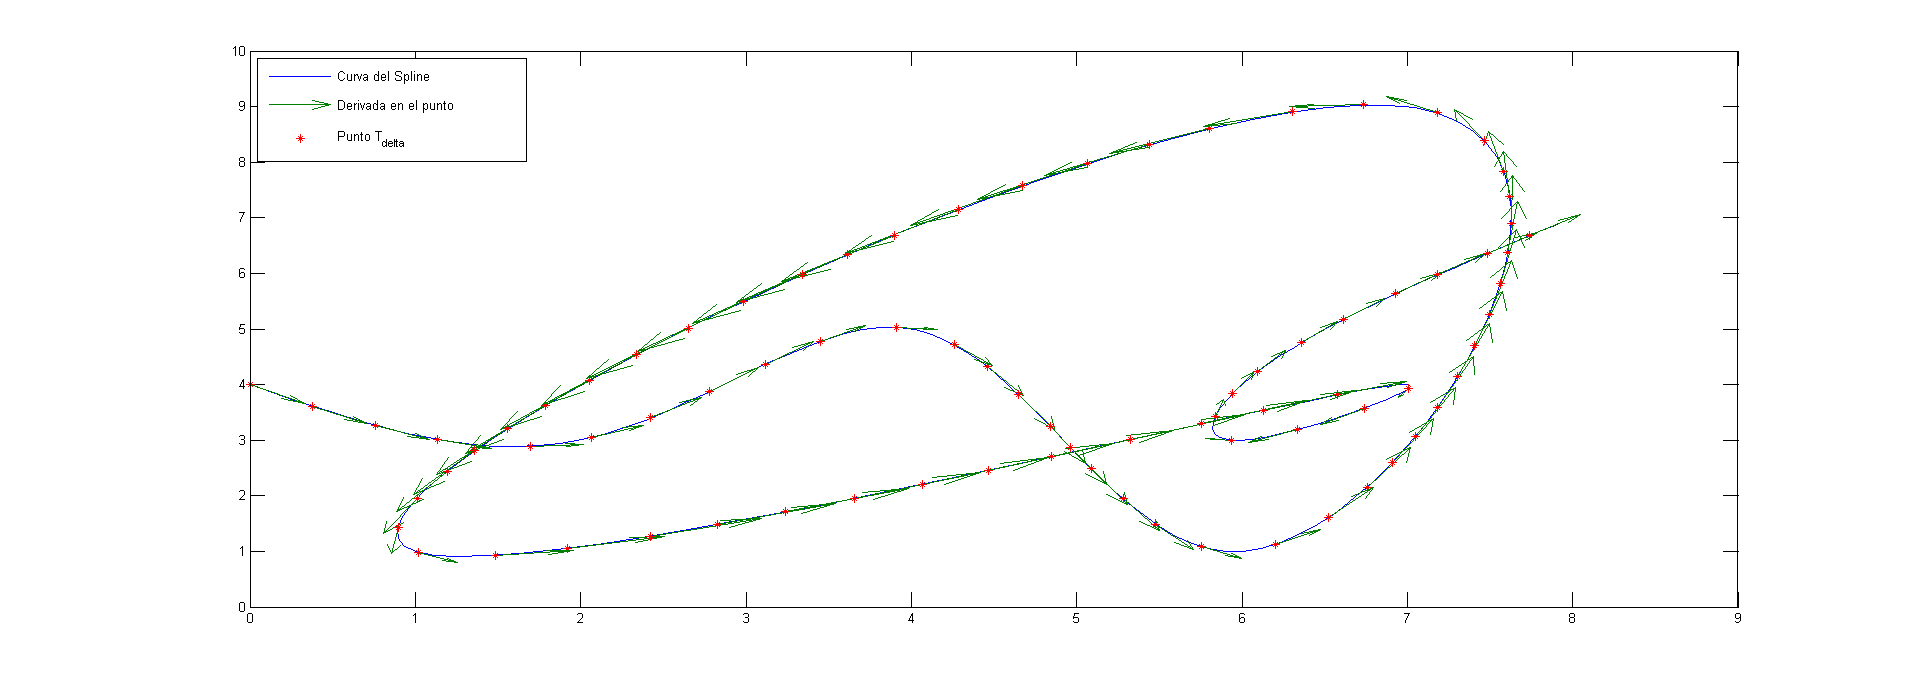
\includegraphics[scale=0.4]{../img/Centripeta-repa-rand.png} \\
\scriptsize{\textsf{\textbf{Gr\'afico 2.3, Spline y reparametrización dada una parametrización centrípeta de los puntos sampleados, con puntos de entrada al azar}}}
\end{center}


Luego se cambió el set de puntos, en lugar de usar un sampleo al azar, se introdujo uno especial que efectúa saltos muy grandes o muy chicos de punto a punto, a manera de ver cómo se comportan las curvas en este caso. Sólo se evaluó la reparametrización, la entrada usada se puede ver en \textit{antiuniforme.txt}


\begin{center}
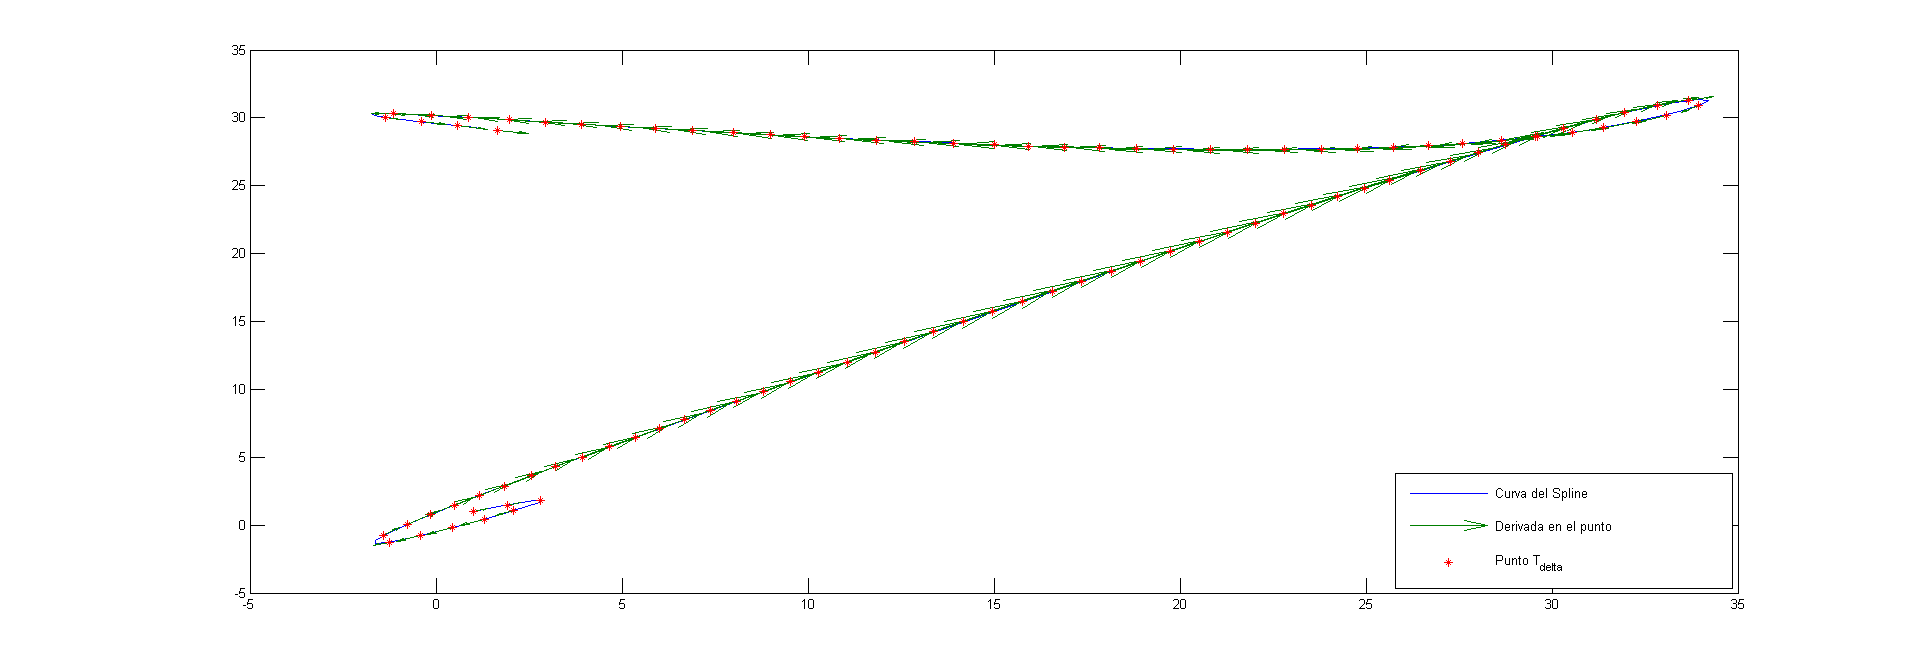
\includegraphics[scale=0.4]{../img/uniforme-antiu.png} \\
\scriptsize{\textsf{\textbf{Gr\'afico 3.1, Spline y reparametrización original dada una parametrización uniforme de los puntos sampleados, con puntos que alternen entre cercanos y lejanos}}}
\end{center}

\begin{center}
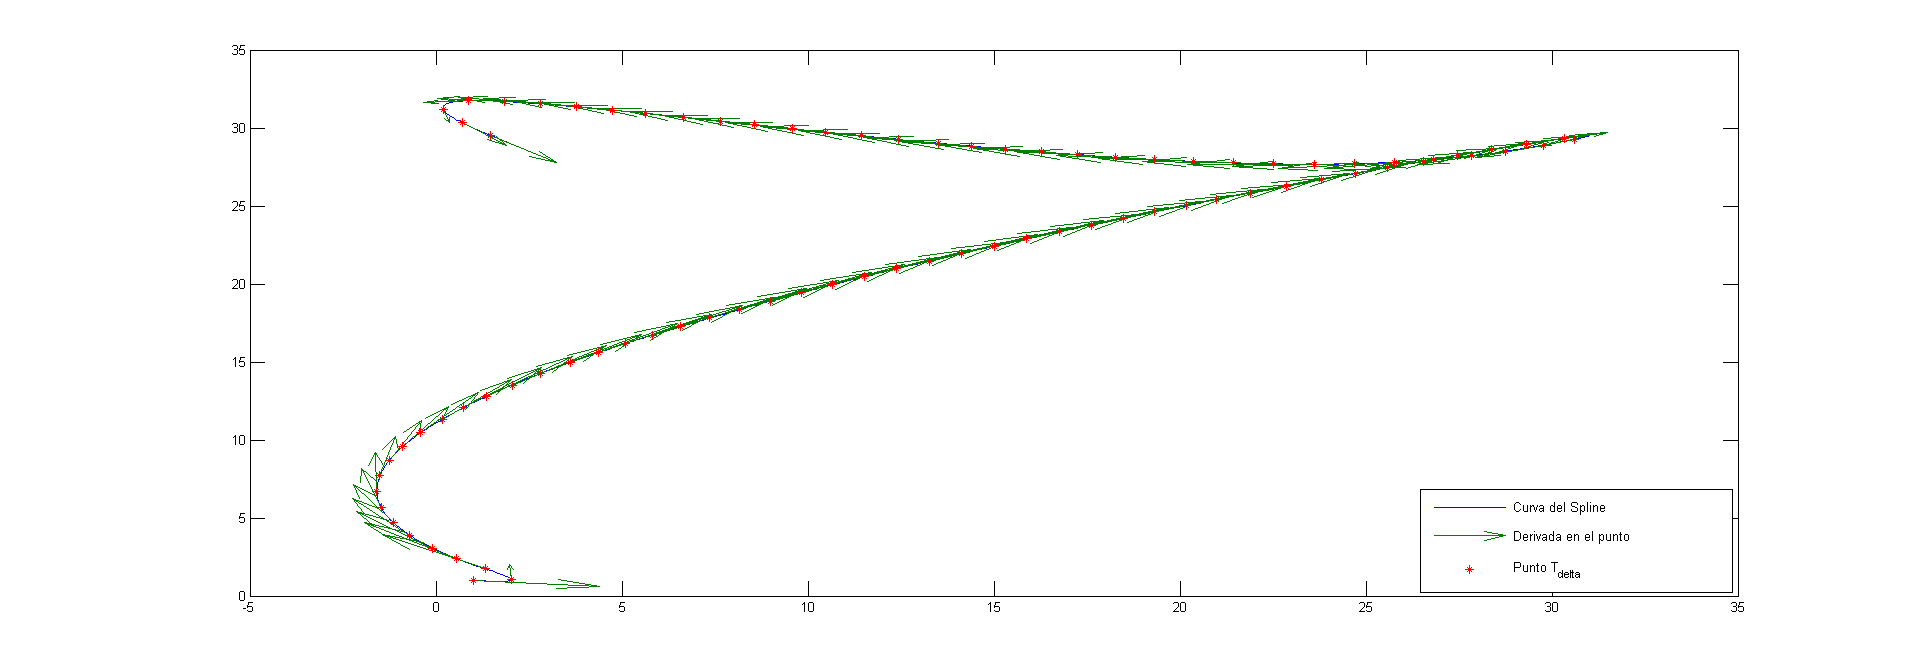
\includegraphics[scale=0.4]{../img/chord-antiu.png} \\
\scriptsize{\textsf{\textbf{Gr\'afico 3.2, Spline y parametrización original dada una parametrización chord-length de los puntos sampleados, con puntos que alternen entre cercanos y}}}
\end{center}

\begin{center}
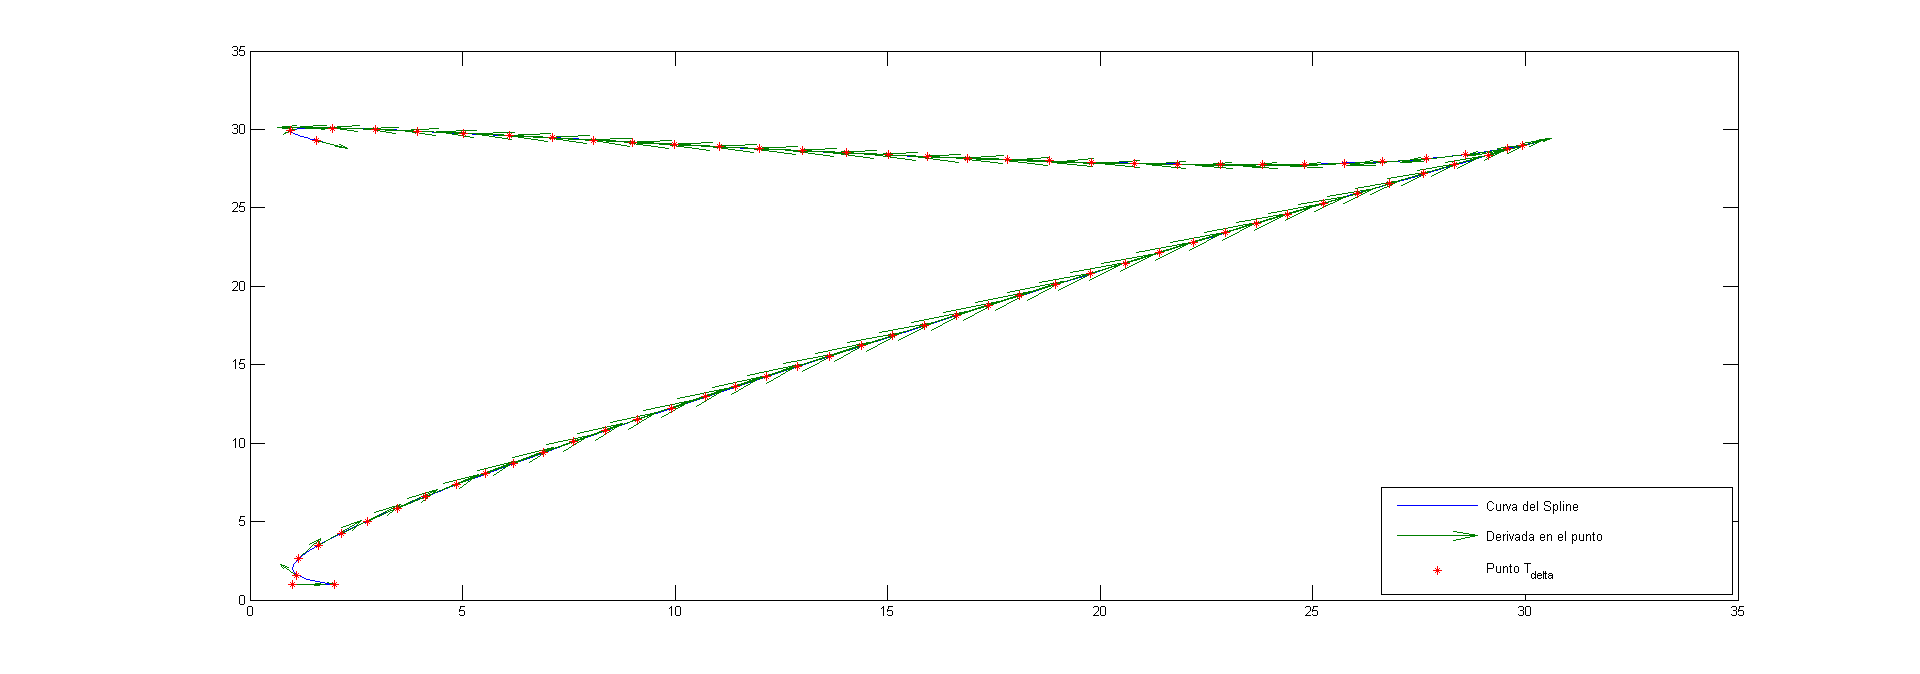
\includegraphics[scale=0.4]{../img/centripeta-antiu.png} \\
\scriptsize{\textsf{\textbf{Gr\'afico 3.3, Spline y parametrización original dada una parametrización centrípeta de los puntos sampleados, con puntos que alternen entre cercanos y}}}
\end{center}


Finalmente, para observar cómo afecta el $\Delta$ al comportamiento, se tomó el mismo \textit{random\_ints.txt} pero cambiando $\Delta$ por 3. Sólo se usó la curva centrípeta para graficar.

\begin{center}
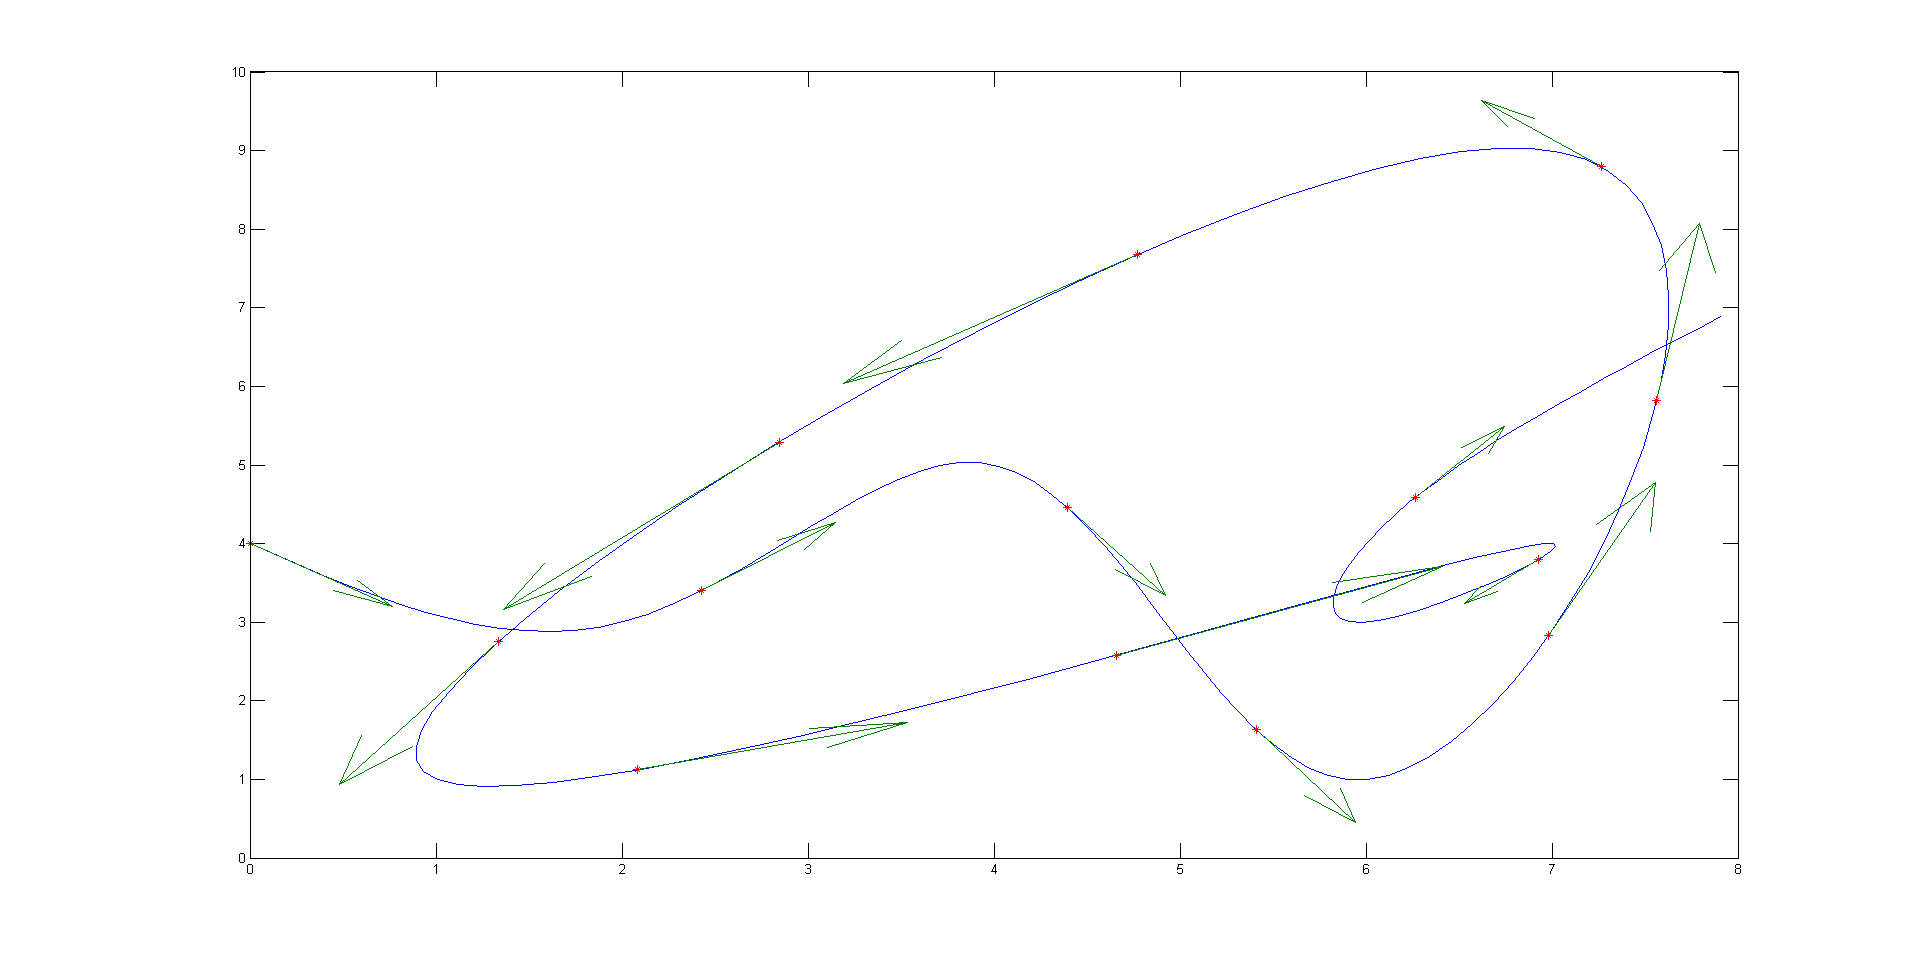
\includegraphics[scale=0.4]{../img/Centripeta-delta3-rand.png} \\
\scriptsize{\textsf{\textbf{Gr\'afico 4.1, Spline y reparametrización dada una parametrización centrípeta de los puntos sampleados, con puntos de entrada al azar, $\Delta = 3$}}}
\end{center}

%%template de como meter un grafico

%\begin{center}
%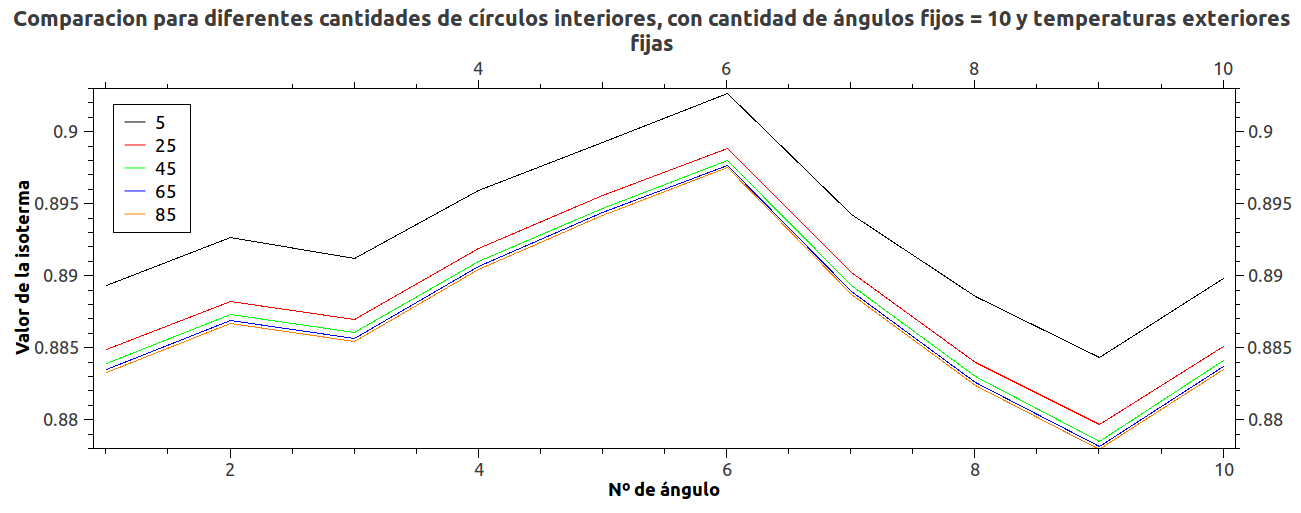
\includegraphics[scale=0.5]{../img/comparacion10ang.png} \\
%\scriptsize{\textsf{\textbf{Gr\'afico 1.1, comparación del comportamiento de la isoterma para
%diferentes cantidades de círculos, con 10 ángulos y temperaturas exteriores fijas}}}
%\end{center}

